\def\iangle{25} % Angle of the inclined plane
\def\down{-90}
\def\arcr{0.5cm} % Radius of the arc used to indicate angles

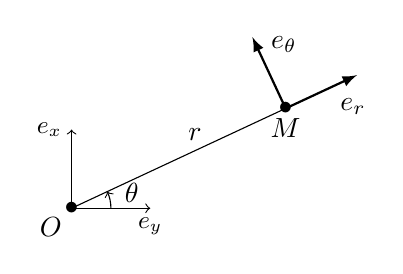
\begin{tikzpicture}[
    force/.style={>=latex,draw=blue,fill=blue},
    base/.style={>=latex},
    axis/.style={font=\small},
    M/.style={rectangle,draw,fill=lightgray,minimum size=0.5cm,thin},
    m/.style={rectangle,draw=black,fill=lightgray,minimum size=0.3cm,thin},
    plane/.style={draw=black,fill=blue!10},
    string/.style={draw=red, thick},
    pulley/.style={thick},
]

%    \draw [ultra thick] (-1,0) -- (1,0) ;%node [midway, above] {$O$};
%    \draw [axis,->] (0,0) -- (0,-3) node [left] {$x$};
    
    \draw (0,0) coordinate (base) -- coordinate[pos=0.5] (mid)++(\iangle:3) coordinate (M) node {$\bullet$} node [below] {$M$}; 
    \draw [->,base, thick] (M) -- ++(\iangle:1) node [xshift = -0.5mm, yshift = -4mm] {$\vv{e_r}$};
    \draw [->,base, thick] (M) -- ++(\iangle+90:1) node [xshift = 4mm, yshift = -1mm] {$\vv{e_\theta}$};
    \draw (mid) node [above right, yshift = 1mm] {$r$};
    
    \draw[->] (base)++(\arcr,0) arc (0:\iangle:\arcr);
    \path (base)++(\iangle-15:\arcr+5pt) node [xshift = 1mm, yshift = 0.75mm] {$\small\theta$};
       
    \coordinate (O) at (0, 0) node {$\bullet$};
    \coordinate (O) at (0, 0) node[below left] {$O$};
    \draw [->,axis] (O) -- ++(1,0) node [below] {$\vv{e_y}$};
    \draw [->,axis] (O) --++ (0,1) node [left] {$\vv{e_x}$};
\end{tikzpicture}
